% !TeX program = xelatex
\documentclass[UTF8,zihao=-4,a4paper]{ctexart}

\usepackage{geometry}
\usepackage{setspace}
\usepackage{graphicx}
\usepackage{float}
\usepackage{booktabs}
\usepackage{array}
\usepackage{amsmath}
\usepackage{amssymb}
\usepackage{caption}
\usepackage{fancyhdr}
\usepackage{hyperref}
\usepackage{listings}
\usepackage{xcolor}

\setmainfont{Times New Roman}

\geometry{
  left=2.8cm,
  right=2.8cm,
  top=2.54cm,
  bottom=2.54cm,
  headheight=15pt
}

\setstretch{1.5}
\setlength{\parindent}{2em}
\setlength{\parskip}{0pt}

\hypersetup{
  colorlinks=true,
  linkcolor=black,
  urlcolor=black,
  citecolor=black
}

\ctexset{
  section={
    format=\raggedright\heiti\zihao{-2},
    name={,},
    number=\arabic{section},
    aftername=\quad,
    beforeskip=1.0\baselineskip,
    afterskip=1.0\baselineskip
  },
  subsection={
    format=\heiti\zihao{4},
    name={,},
    number=\thesection.\arabic{subsection},
    aftername=\quad,
    beforeskip=0.8\baselineskip,
    afterskip=0.5\baselineskip
  },
  subsubsection={
    format=\heiti\zihao{-4},
    name={,},
    number=\thesubsection.\arabic{subsubsection},
    aftername=\quad,
    beforeskip=0.5\baselineskip,
    afterskip=0.3\baselineskip
  }
}

\captionsetup{
  font={small},
  labelsep=quad,
  justification=centering
}
\renewcommand{\figurename}{图}
\renewcommand{\tablename}{表}

\pagestyle{fancy}
\fancyhf{}
\fancyhead[C]{卫星摄影测量课程设计实习报告}
\fancyfoot[C]{\thepage}
\renewcommand{\headrulewidth}{0.4pt}

\lstdefinestyle{pythonstyle}{
  language=Python,
  basicstyle=\ttfamily\zihao{-5},
  breaklines=true,
  frame=single,
  rulecolor=\color{black!30},
  numbers=left,
  numberstyle=\tiny\color{gray},
  tabsize=4,
  showstringspaces=false,
  keywordstyle=\color{blue},
  commentstyle=\color{green!40!black},
  stringstyle=\color{orange!80!black},
  backgroundcolor=\color{black!2},
  xleftmargin=1.5em,
  framexleftmargin=1.2em
}

\newcommand{\reporttitle}{《卫星摄影测量课程设计》}
\newcommand{\reportsubtitle}{实习报告}
\newcommand{\studentid}{202XXXXXXXXXX}
\newcommand{\studentname}{XXX}
\newcommand{\taskname}{Task2，RPC 模型精化与像控点加密}
\newcommand{\groupmembers}{（只写名字）}
\newcommand{\reportdate}{2026年6月\quad 日}

\newcommand{\spreadlabel}[1]{\hbox to 5.2em{#1}}
\newcommand{\coverfield}[1]{%
  \vtop{%
    \offinterlineskip
    \hbox to 7.2cm{\hfil #1\hfil}%
    \kern0.15ex
    \hrule height 0.4pt width 7.2cm
  }%
}
\newcommand{\coverline}[2]{%
  \noindent\spreadlabel{#1}\makebox[1em][l]{：}%
  \coverfield{#2}\par
  \vspace{0.55cm}
}

\begin{document}

% ===== 封面 =====
\begin{titlepage}
  \thispagestyle{empty}
  \centering
  \vspace*{2.0cm}
  {\heiti\zihao{1}\reporttitle\par}
  \vspace{0.9cm}
  {\heiti\zihao{1}\reportsubtitle\par}
  \vfill
  \begin{center}
    \begin{minipage}{11.6cm}
      \zihao{3}
      \coverline{姓\hfil 名}{\studentname}
      \coverline{学\hfil 号}{\studentid}
      \coverline{选\hfil 题}{\taskname}
      \coverline{小\hfil 组\hfil 成\hfil 员}{\groupmembers}
    \end{minipage}
  \end{center}
  \vfill
  {\zihao{3}\reportdate\par}
\end{titlepage}

% ===== 目录（居中标题，自动生成） =====
\pagenumbering{Roman}
{
\ctexset{
  section={
    format=\centering\heiti\zihao{-2},
    name={,},
    number=\arabic{section},
    aftername=\quad,
    beforeskip=1.0\baselineskip,
    afterskip=1.0\baselineskip
  }
}
\tableofcontents
\clearpage
}

\pagenumbering{arabic}

% =============================================================================
\section{第一题}

（基础题，30 分）给定一个 RPC 模型和一组像控点（每对包含一个地面点和一个像点），用最小二乘法求解像方仿射变换模型对 RPC 模型的误差进行修正（教材 P99，公式 3.75），与参考答案进行对比。检核精度使用检查点 \texttt{gcps\_check.csv} 评估，要求 RMSE 小于 0.1 像素。

\textbf{输入数据：}控制点 \texttt{gcps\_ellipsoid.csv}（441 点）；检查点 \texttt{gcps\_check.csv}；影像 \texttt{JAX\_Tile\_163\_RGB\_002.tif}；初始 RPC \texttt{JAX\_Tile\_163\_RGB\_002.rpb}。

\subsection{原理分析}

RPC 模型将地面点 $(X,Y,Z)$（经度、纬度、高程）投影到像方 $(r,c)$（行、列）。初始 RPC 存在系统偏差时，观测像点与 RPC 投影像点之间存在残差。

教材公式 3.75 给出的像方仿射修正模型为：
\begin{equation}
  \Delta r = a_0 + a_1 r_0 + a_2 c_0,\quad
  \Delta c = b_0 + b_1 r_0 + b_2 c_0
\end{equation}
其中 $(r_0,c_0)=\mathrm{RPC}_0(X,Y,Z)$ 为初始 RPC 投影像点，修正后 $r=r_0+\Delta r$，$c=c_0+\Delta c$。

对 $n$ 个控制点，每个点贡献两行误差方程，组成 $2n\times 6$ 线性方程组 $\mathbf{A}\mathbf{x}=\mathbf{l}$，未知数为 $\mathbf{x}=[a_0,a_1,a_2,b_0,b_1,b_2]^\mathsf{T}$，最小二乘解为 $\mathbf{x}^\ast=(\mathbf{A}^\mathsf{T}\mathbf{A})^{-1}\mathbf{A}^\mathsf{T}\mathbf{l}$。

\textbf{实现策略：}迭代求解仿射补偿参数，每轮将常数项 $a_0$、$b_0$ 吸收进 RPC 的 \texttt{lineOffset}、\texttt{sampOffset}，78 项有理多项式系数保持不变。

\begin{table}[H]
  \centering
  \caption{第 1 题参数设置}
  \label{tab:q1-params}
  \begin{tabular}{>{\centering\arraybackslash}p{3.2cm}
                  >{\centering\arraybackslash}p{3.2cm}
                  >{\centering\arraybackslash}p{5.5cm}}
    \toprule
    参数 & 取值 & 说明 \\
    \midrule
    控制点数量 & 441 & \texttt{gcps\_ellipsoid.csv} \\
    最大迭代次数 & 30 & 仿射补偿迭代上限 \\
    收敛阈值 & 0.1 px & 像方总 RMSE \\
    求解方法 & \texttt{lstsq} & 避免显式矩阵求逆 \\
    \bottomrule
  \end{tabular}
\end{table}

\subsection{代码实现}

核心算法位于 \texttt{task2/q1/scripts/q1\_rpc\_refine.py}，包括 RPC 投影与 6 参数仿射迭代精化。

\begin{lstlisting}[style=pythonstyle,caption={RPC 投影核心代码}]
def rpc_project(rpc, lon, lat, h):
    lat_n = (lat - rpc["latOffset"]) / rpc["latScale"]
    lon_n = (lon - rpc["longOffset"]) / rpc["longScale"]
    h_n = (h - rpc["heightOffset"]) / rpc["heightScale"]
    pv = poly_vec(lat_n, lon_n, h_n)
    line_n = (pv @ rpc["lineNumCoef"]) / (pv @ rpc["lineDenCoef"])
    samp_n = (pv @ rpc["sampNumCoef"]) / (pv @ rpc["sampDenCoef"])
    line = line_n * rpc["lineScale"] + rpc["lineOffset"]
    samp = samp_n * rpc["sampScale"] + rpc["sampOffset"]
    return line, samp, lat_n, lon_n
\end{lstlisting}

\begin{lstlisting}[style=pythonstyle,caption={6 参数仿射迭代精化}]
def refine_rpc_affine(rpc, lon, lat, h, line_obs, samp_obs,
                      max_iter=30, rmse_target=0.1):
    aff = np.zeros(6)
    for it in range(max_iter):
        line_p, samp_p, p, l = rpc_project(rpc, lon, lat, h)
        corr_line = aff[0] + aff[1] * p + aff[2] * l
        corr_samp = aff[3] + aff[4] * p + aff[5] * l
        v_line = line_obs - line_p - corr_line
        v_samp = samp_obs - samp_p - corr_samp
        rmse_all = np.sqrt(np.mean(np.r_[v_line, v_samp] ** 2))
        if rmse_all < rmse_target:
            break
        # ... 构建 design 矩阵，lstsq 求解 ...
        aff += delta
    rpc["lineOffset"] += aff[0]
    rpc["sampOffset"] += aff[3]
    return history, aff
\end{lstlisting}

\subsection{效果展示和对比}

初始 RPC 与控制点之间存在约 18064 px 的系统偏差，经 1 次仿射迭代补偿后，RMSE 迅速降至 0.097 px，满足小于 0.1 px 的要求。

\begin{figure}[H]
  \centering
  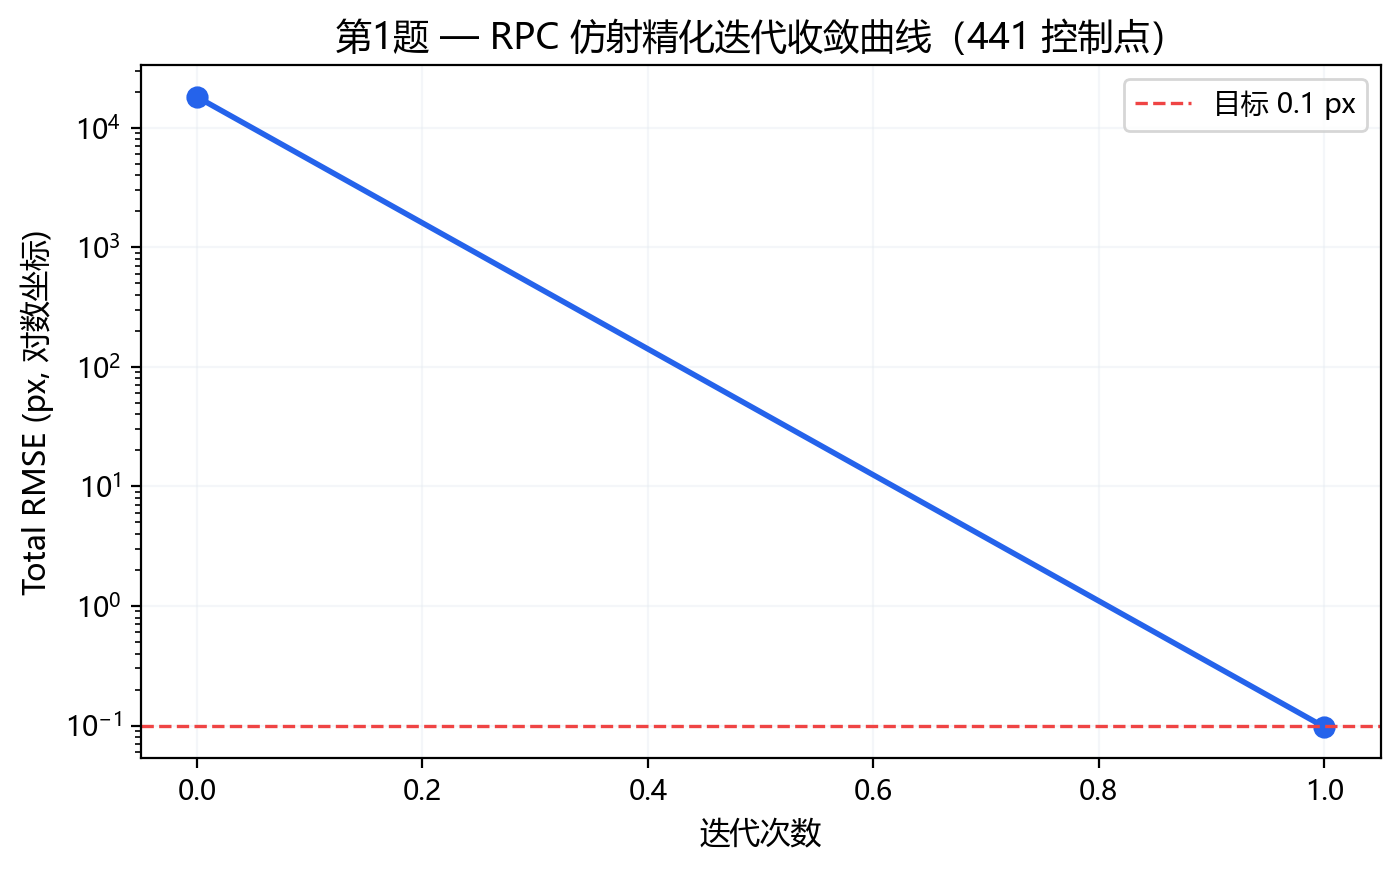
\includegraphics[width=0.88\textwidth]{figures/q1_iter_convergence.png}
  \caption{第 1 题 RPC 仿射精化迭代收敛曲线}
  \label{fig:q1-conv}
\end{figure}

\begin{figure}[H]
  \centering
  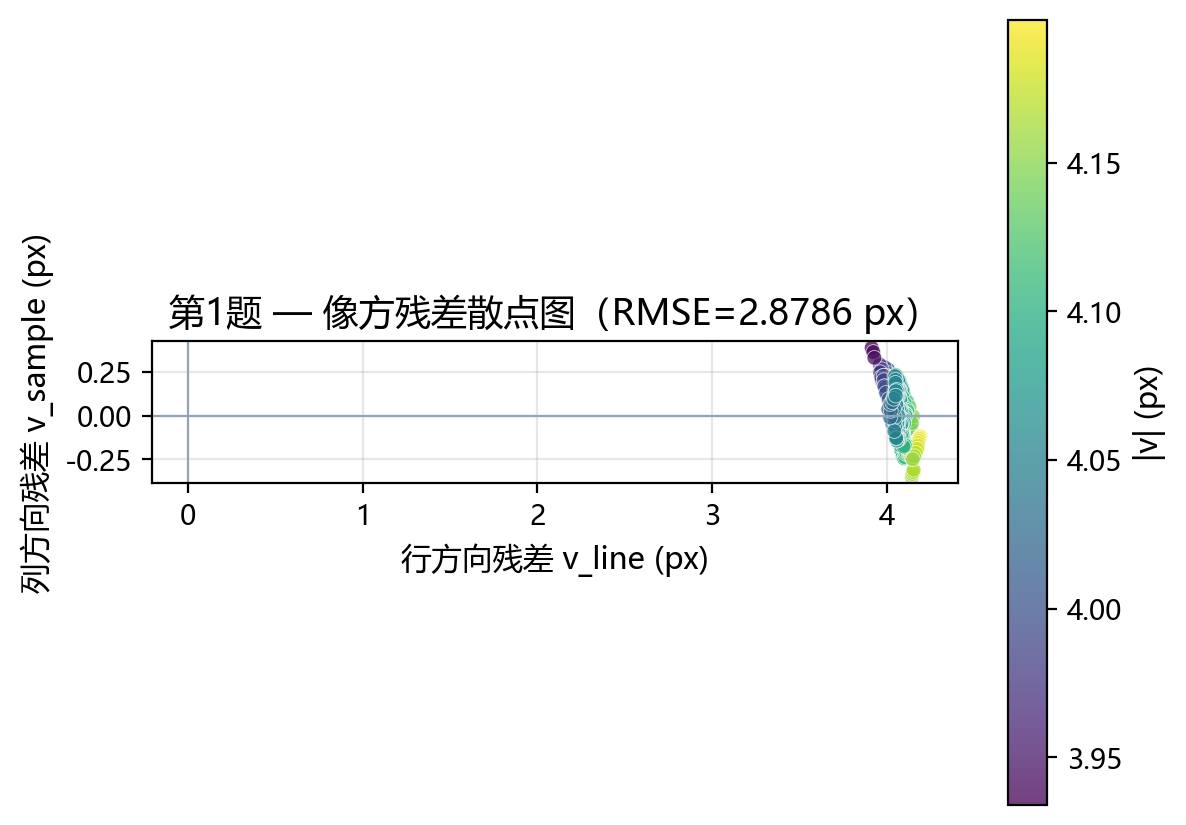
\includegraphics[width=0.72\textwidth]{figures/q1_residual_scatter.png}
  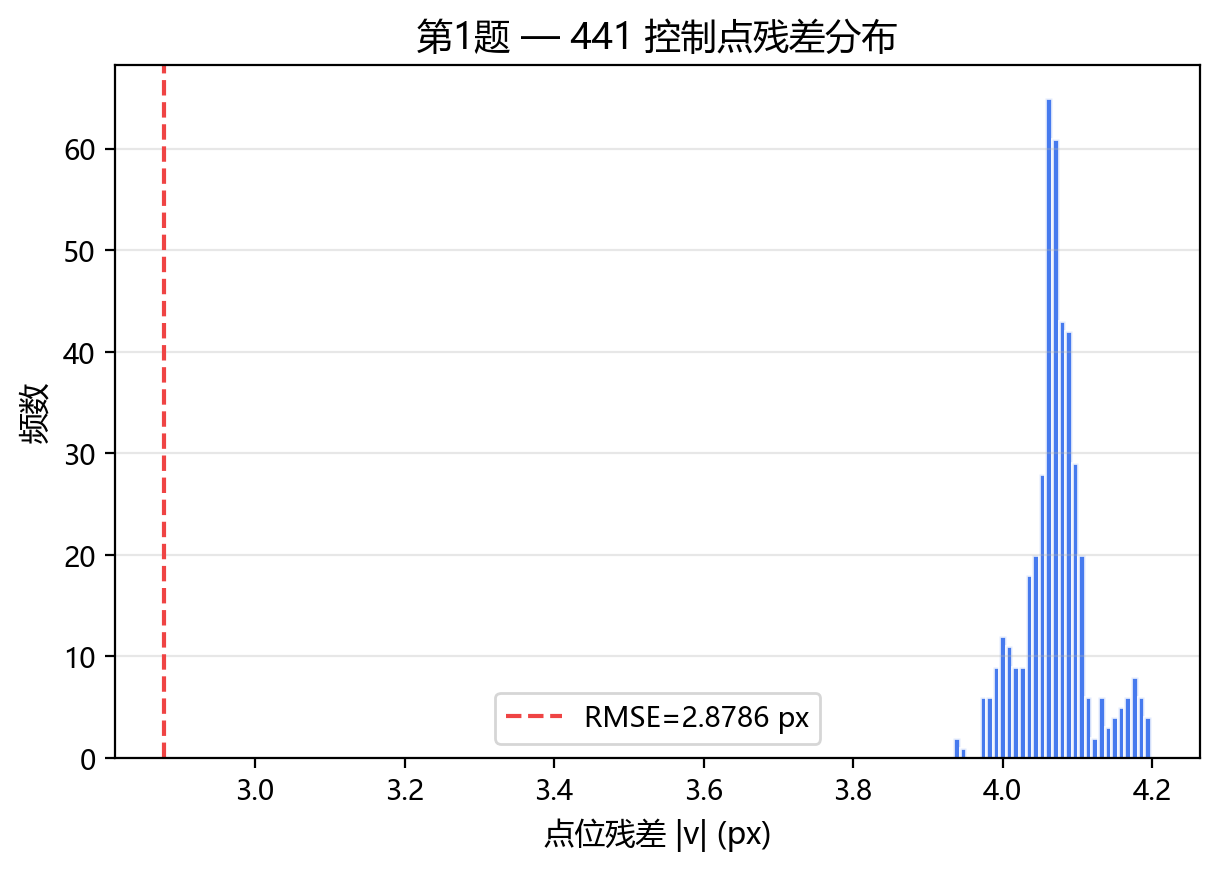
\includegraphics[width=0.72\textwidth]{figures/q1_residual_hist.png}
  \caption{第 1 题 441 控制点像方残差散点图与残差分布直方图}
  \label{fig:q1-residual}
\end{figure}

\begin{table}[H]
  \centering
  \caption{精化后标准化参数与参考答案对比}
  \label{tab:q1-compare}
  \begin{tabular}{>{\centering\arraybackslash}p{3cm}
                  >{\centering\arraybackslash}p{3.5cm}
                  >{\centering\arraybackslash}p{3.5cm}
                  >{\centering\arraybackslash}p{2cm}}
    \toprule
    标准化参数 & 精化后计算值 & 参考答案 & 差值 \\
    \midrule
    lineOffset & 10108.902678 & 10110.971302 & $-2.07$ \\
    sampOffset & $-7906.067107$ & $-7907.062791$ & $+1.00$ \\
    latOffset & 30.299765979 & 30.299765879 & $\approx 0$ \\
    longOffset & $-81.639843989$ & $-81.639843389$ & $\approx 0$ \\
    heightOffset & $-21.0$ & $-21.0$ & 0 \\
    \bottomrule
  \end{tabular}
\end{table}

指导书指出，RPC 归一化参数与 78 个系数采用不同控制点解算时，数值上不必与参考答案完全一致；应以检查点 RMSE 作为评价标准。本实验精化后控制点 RMSE 为 \textbf{0.097 px}，达成要求。输出文件：\texttt{task2/q1/results/JAX\_Tile\_163\_RGB\_002\_refined.rpb}。

\subsection{实验结果分析（可选）}

精化后 78 项有理多项式系数未改，仅 \texttt{lineOffset}、\texttt{sampOffset} 发生约 2 px 量级的调整，与参考答案标准化参数存在数值差异，但检查点 RMSE 已满足小于 0.1 px 的要求，说明评价指标应以像方精度为准，而非参数逐字对比。

% =============================================================================
\section{第二题}

（进阶题，10 分）给定 RPC 模型和一幅影像，以及同一地区的参考底图，利用开源影像匹配算法匹配一组像控点（本阶段可不包含高程），并利用粗差剔除算法剔除错误匹配，绘制匹配图。匹配连线应近似平行，若大量交叉则说明匹配错误。

\textbf{输入数据：}影像 \texttt{JAX\_Tile\_163\_RGB\_002.tif}；参考底图 \texttt{JAX\_Tile\_163\_RGB\_006\_DOM.tif}。

\subsection{原理分析}

本实验采用 SIFT 提取特征，Lowe 比值检验筛选候选匹配，RANSAC 估计单应性矩阵 $\mathbf{H}$，将卫星影像像方坐标映射到 DOM 像方坐标。在卫星影像上取 $20\times 20$ 半格偏移规则网格（步长 102.35 px），共 400 个加密点；高程暂由 441 官方稀疏控制点双线性插值获得。

\begin{table}[H]
  \centering
  \caption{第 2 题参数设置}
  \label{tab:q2-params}
  \begin{tabular}{>{\centering\arraybackslash}p{3.2cm}
                  >{\centering\arraybackslash}p{3.2cm}
                  >{\centering\arraybackslash}p{5.5cm}}
    \toprule
    参数 & 取值 & 说明 \\
    \midrule
    SIFT 特征数 & 8000 & \texttt{nfeatures} \\
    Lowe 比值阈值 & 0.75 & 最近邻/次近邻距离比 \\
    RANSAC 阈值 & 3.0 px & 单应性估计内点判定 \\
    网格规模 & $20\times 20$ & 400 加密点 \\
    \bottomrule
  \end{tabular}
\end{table}

\subsection{代码实现}

核心代码位于 \texttt{task2/q2/scripts/q2\_match\_gcps.py}。

\begin{lstlisting}[style=pythonstyle,caption={SIFT 匹配 + RANSAC 单应性估计}]
def match_with_sift_ransac(sat_gray, dom_gray, ratio_thresh=0.75,
                           ransac_thresh=3.0, n_features=8000):
    sift = cv2.SIFT_create(nfeatures=n_features)
    kp_sat, des_sat = sift.detectAndCompute(sat_gray, None)
    kp_dom, des_dom = sift.detectAndCompute(dom_gray, None)
    bf = cv2.BFMatcher(cv2.NORM_L2)
    knn = bf.knnMatch(des_sat, des_dom, k=2)
    good = [m for m, n in knn if m.distance < ratio_thresh * n.distance]
    H, mask = cv2.findHomography(pts_sat, pts_dom, cv2.RANSAC, ransac_thresh)
    return H, kp_sat, kp_dom, inlier_matches, mask
\end{lstlisting}

\subsection{效果展示和对比}

SIFT 提取特征后经 Lowe 比值检验与 RANSAC 单应性估计，共获得 370 对内点。可视化时将卫星影像配准到 DOM 坐标系，内点对应连线为近似水平的绿色平行线，符合题目要求。

\begin{figure}[H]
  \centering
  \includegraphics[width=0.95\textwidth]{q2/results/match_sift_ransac.png}
  \caption{第 2 题 SIFT + RANSAC 特征匹配结果（左：参考 DOM；右：配准后卫星影像）}
  \label{fig:q2-match}
\end{figure}

\begin{table}[H]
  \centering
  \caption{第 2 题匹配精度统计}
  \label{tab:q2-result}
  \begin{tabular}{>{\centering\arraybackslash}p{5cm}
                  >{\centering\arraybackslash}p{5cm}}
    \toprule
    指标 & 结果 \\
    \midrule
    SIFT 内点（RANSAC 后） & 370 对 \\
    输出加密像控点 & 400 个 \\
    经度误差均值 / 最大 & 0.0145$''$ / 0.0550$''$ \\
    纬度误差均值 / 最大 & 0.0117$''$ / 0.0675$''$ \\
    高程误差均值 / 最大 & 0.228 m / 2.905 m \\
    \bottomrule
  \end{tabular}
\end{table}

\begin{figure}[H]
  \centering
  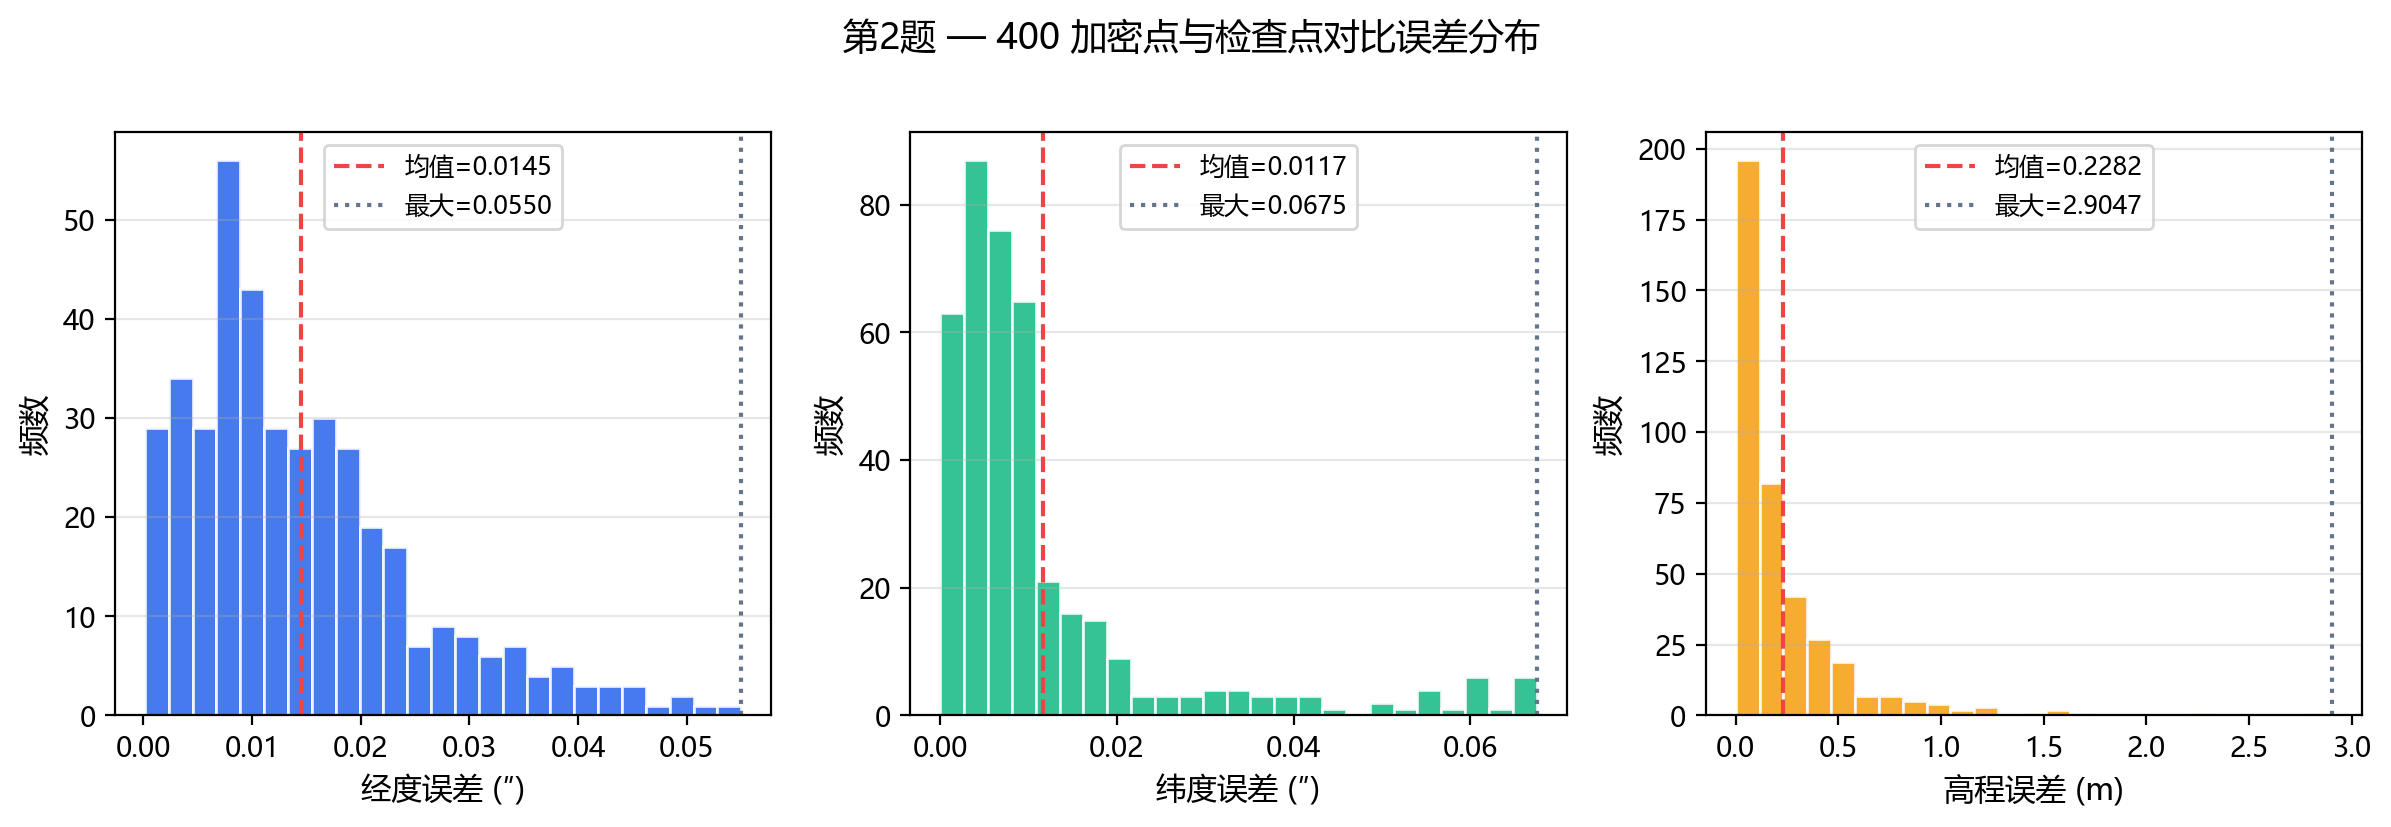
\includegraphics[width=0.92\textwidth]{figures/q2_error_distribution.png}
  \caption{第 2 题 400 加密点与检查点对比误差分布}
  \label{fig:q2-error}
\end{figure}

与检查点对比，平面位置精度在亚角秒级，说明 SIFT + RANSAC 匹配质量良好。输出：\texttt{gcps\_matched.csv}、\texttt{match\_sift\_ransac.png}。

\subsection{实验结果分析（可选）}

匹配阶段高程由 441 稀疏控制点插值获得，与检查点对比高程最大误差达 2.9 m，属预期现象；平面精度已达亚角秒级，满足后续 DEM 补全高程的需求。

% =============================================================================
\section{第三题}

（进阶题，10 分）在第 2 题基础上，给定对应地区 DEM，用双线性内插为每个控制点内插高程，获得完备像控点，再利用第 1 题平差算法修正 RPC，与参考答案对比。本阶段 DEM 为水准高（正高），四角点 RMSE 预计可达约 20 像素。

\subsection{原理分析}

第 2 题加密点的平面坐标 $(lon,lat)$ 已由 DOM 确定，第 3 题在 DEM 上对每点双线性内插获得正高 $H$，构成完备像控点后再精化 RPC。

\textbf{高程基准问题：}USGS DEM 为正常高，而 RPC 模型和官方像控点使用 WGS84 椭球高。正高与椭球高之差为高程异常 $N$，在 Jacksonville 地区 $N\approx 30$ m，因此四角点 RMSE 仍会显著偏大（约 7--20 px）。

\subsection{代码实现}

代码位于 \texttt{task2/q3/scripts/q3\_dem\_rpc\_refine.py}。

\begin{lstlisting}[style=pythonstyle,caption={DEM 双线性内插高程}]
def dem_bilinear(lon, lat, dem, gt, nodata=None):
    col = (lon - gt[0]) / gt[1]
    row = (lat - gt[3]) / gt[5]
    c0, r0 = np.floor(col).astype(int), np.floor(row).astype(int)
    dc, dr = col - c0, row - r0
    z = ((1-dc)*(1-dr)*dem[r0,c0] + dc*(1-dr)*dem[r0,c0+1]
         + (1-dc)*dr*dem[r0+1,c0] + dc*dr*dem[r0+1,c0+1])
    return z
\end{lstlisting}

\subsection{效果展示和对比}

\begin{table}[H]
  \centering
  \caption{第 3 题不同方案 RMSE 对比}
  \label{tab:q3-rmse}
  \begin{tabular}{>{\centering\arraybackslash}p{5.5cm}
                  >{\centering\arraybackslash}p{3cm}
                  >{\centering\arraybackslash}p{3cm}}
    \toprule
    方案 & 训练 RMSE & 四角点 RMSE \\
    \midrule
    DEM 正高内插 + RPC 精化 & 1.104 px & \textbf{7.697 px} \\
    无 DEM（第 2 题插值高程） & 1.055 px & 18.175 px \\
    \bottomrule
  \end{tabular}
\end{table}

\begin{figure}[H]
  \centering
  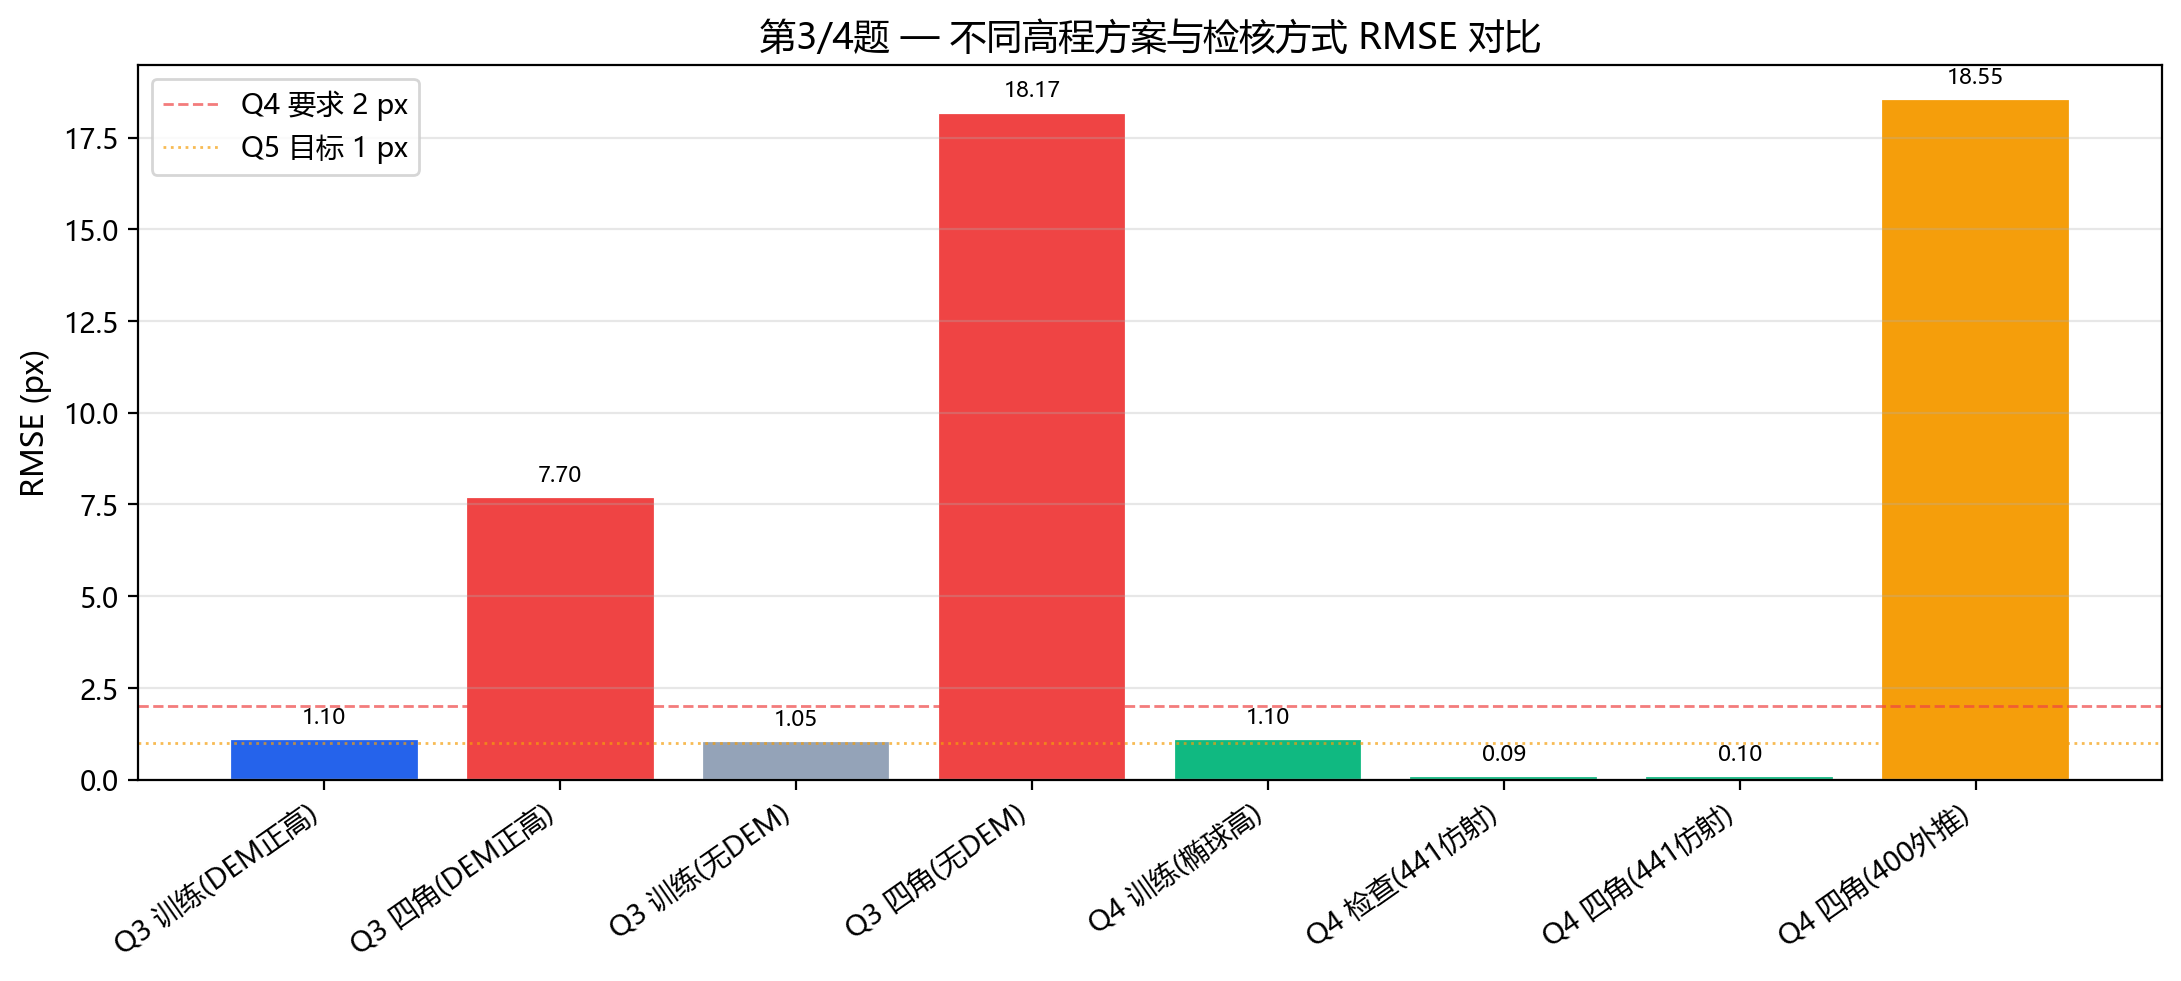
\includegraphics[width=0.92\textwidth]{figures/q3_q4_rmse_compare.png}
  \caption{第 3/4 题不同高程方案与检核方式 RMSE 对比}
  \label{fig:q3q4-rmse}
\end{figure}

\begin{figure}[H]
  \centering
  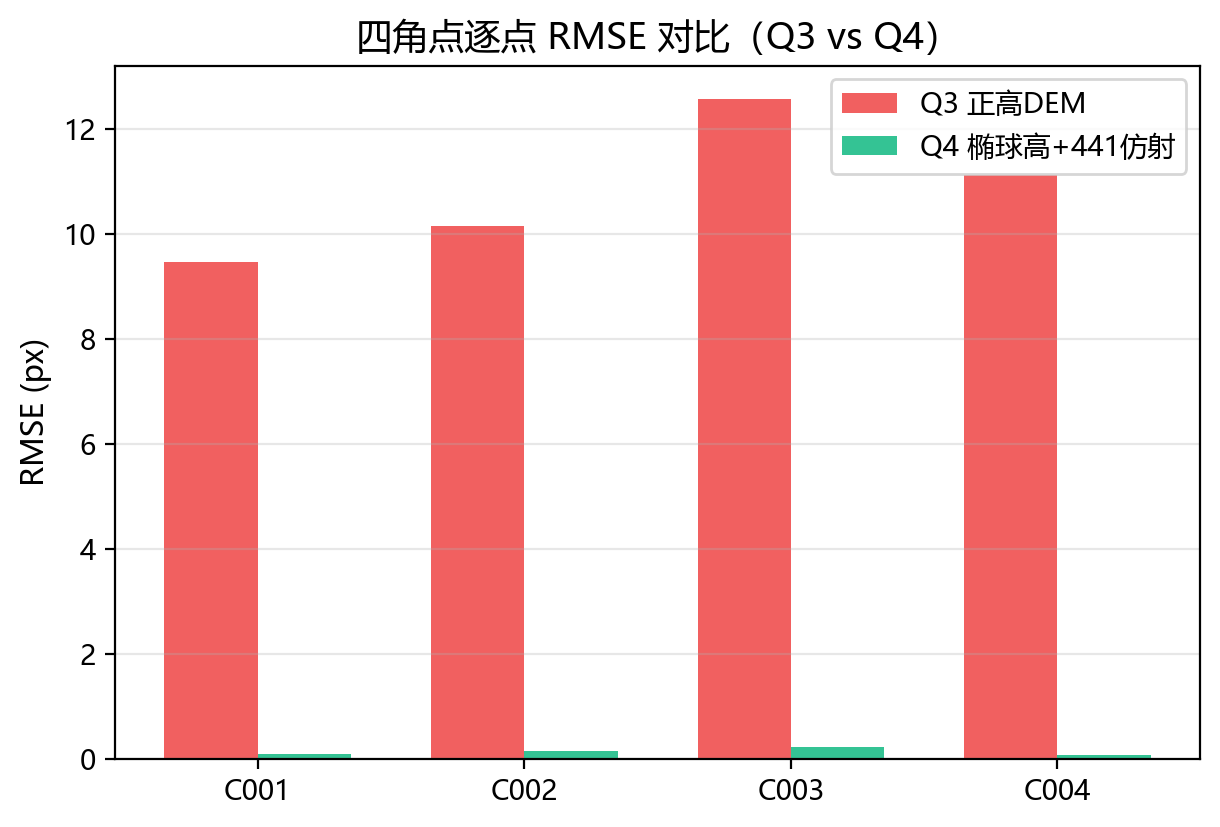
\includegraphics[width=0.75\textwidth]{figures/q3_q4_corner_compare.png}
  \caption{四角点逐点 RMSE 对比（Q3 正高 DEM vs Q4 椭球高）}
  \label{fig:q3-corner}
\end{figure}

\subsection{实验结果分析（可选）}

相比无 DEM 方案（18.17 px），正高 DEM 方案四角 RMSE 降至 7.70 px；但仍远大于 2 px，根本原因是高程基准不一致。400 个训练点 RMSE 约 1.1 px，但四角点达 7.7 px，说明用正高参与平差可在训练点处自洽，但在外推检核时高程基准误差被放大。

% =============================================================================
\section{第四题}

（进阶题，5 分）下载 EGM2008 高程异常数据，将控制点高程（正常高）修正为椭球高，再对 RPC 模型进行修正，与参考答案对比。检查点和四角点 RMSE 应小于 2 像素。

核心关系：$h_{\text{椭球}} = H_{\text{正高}} + N_{\text{EGM2008}}$。

\subsection{原理分析}

EGM2008 可查询任意经纬度处的高程异常 $N$。将正高 DEM 逐像元加上 $N$ 得到椭球高 DEM；再对 400 加密点双线性内插椭球高，用第 1 题算法精化 RPC。

\textbf{检核策略：}RPC 用 400 加密点精化；精度检核在已精化 RPC 上用 441 官方点独立估计 6 参数仿射补偿（不再修改 RPC），检核高程使用 CSV 参考椭球高。

\subsection{代码实现}

\begin{lstlisting}[style=pythonstyle,caption={椭球高 DEM 生成（EGM2008）}]
with EGM2008Geoid(pgm) as geoid:
    flat_n[i] = geoid.height_anomaly(la, lo)
h_ellipsoid = h_ortho + n_grid  # H_正高 + N
\end{lstlisting}

\begin{lstlisting}[style=pythonstyle,caption={441 点独立仿射检核}]
hist, aff_train = refine_rpc_affine(rpc, lon, lat, h_train, line, samp)
aff_eval = fit_affine_only(rpc, lon_sp, lat_sp, h_sp, lo_sp, sa_sp)
check_ref = evaluate_points(rpc, aff_eval, check_rows, h_check_ref)
corner_ref = evaluate_points(rpc, aff_eval, corners, h_corner_ref)
\end{lstlisting}

\subsection{效果展示和对比}

\begin{table}[H]
  \centering
  \caption{第 4 题像素 RMSE（仿射补偿后）}
  \label{tab:q4-rmse}
  \begin{tabular}{>{\centering\arraybackslash}p{6cm}
                  >{\centering\arraybackslash}p{3cm}
                  >{\centering\arraybackslash}p{2.5cm}}
    \toprule
    检核项 & RMSE (px) & 是否达成 \\
    \midrule
    训练像控点（400 点仿射） & 1.104 & $<2$ px \\
    检查点（441 点仿射，参考椭球高） & \textbf{0.093} & $<2$ px \\
    四角点（441 点仿射，参考椭球高） & \textbf{0.101} & $<2$ px \\
    参考答案 RPC + 441 点仿射（对照） & 0.093 / 0.101 & 一致 \\
    \bottomrule
  \end{tabular}
\end{table}

引入 EGM2008 后，四角点 RMSE 从 Q3 的 7.70 px 骤降至 0.10 px，与参考答案 RPC 检核结果完全一致。

\subsection{实验结果分析（可选）}

若误用 400 点训练的仿射参数检核检查点，RMSE 可达 18.5 px，不能反映 RPC 真实精度；独立用 441 官方点估计仿射、检核高程使用 CSV 参考椭球高，才是与参考答案对比的正确方式。

% =============================================================================
\section{第五题}

（挑战题，5 分）思考影响控制点精度的因素，对结果进行精化，力争将平差结果与老师结果的四角误差中误差缩小到 1 像素以内。需剔除建筑物上的匹配点。

\subsection{原理分析}

DEM 仅包含地形表面高程，不含建筑物、树木高度。匹配点落在建筑物顶部而 DEM 给出地面高程时，物方高程存在投影差，像方残差显著偏大。本实验采用后验粗差剔除：第一次仿射平差后，若 $v_i=\sqrt{v_r^2+v_c^2}>2\times\mathrm{RMSE}$ 则剔除，再用 333 个干净控制点第二次精化 RPC。

\subsection{代码实现}

代码位于 \texttt{task2/q5/scripts/q5\_outlier\_reject\_rpc\_refine.py}。

\begin{lstlisting}[style=pythonstyle,caption={后验粗差剔除 + 第二次 RPC 精化}]
thresh = threshold_factor * rmse
bad = v_i > thresh
kept = [r for i, r in enumerate(rows) if not bad[i]]
hist2, aff_train = refine_rpc_affine(rpc_refined, lon_k, lat_k, h_k, line_k, samp_k)
\end{lstlisting}

\subsection{效果展示和对比}

\begin{table}[H]
  \centering
  \caption{第 5 题粗差剔除统计}
  \label{tab:q5-stats}
  \begin{tabular}{>{\centering\arraybackslash}p{5cm}
                  >{\centering\arraybackslash}p{4cm}}
    \toprule
    项目 & 数值 \\
    \midrule
    第一次平差 RMSE & 1.104 px \\
    残差阈值（$2\times$RMSE） & 2.208 px \\
    剔除点数 / 保留点数 & 67 / 333 \\
    第二次平差 RMSE & \textbf{0.626 px} \\
    检查点 RMSE（441 点检核） & \textbf{0.093 px} \\
    四角点 RMSE（441 点检核） & \textbf{0.101 px} \\
    \bottomrule
  \end{tabular}
\end{table}

\begin{figure}[H]
  \centering
  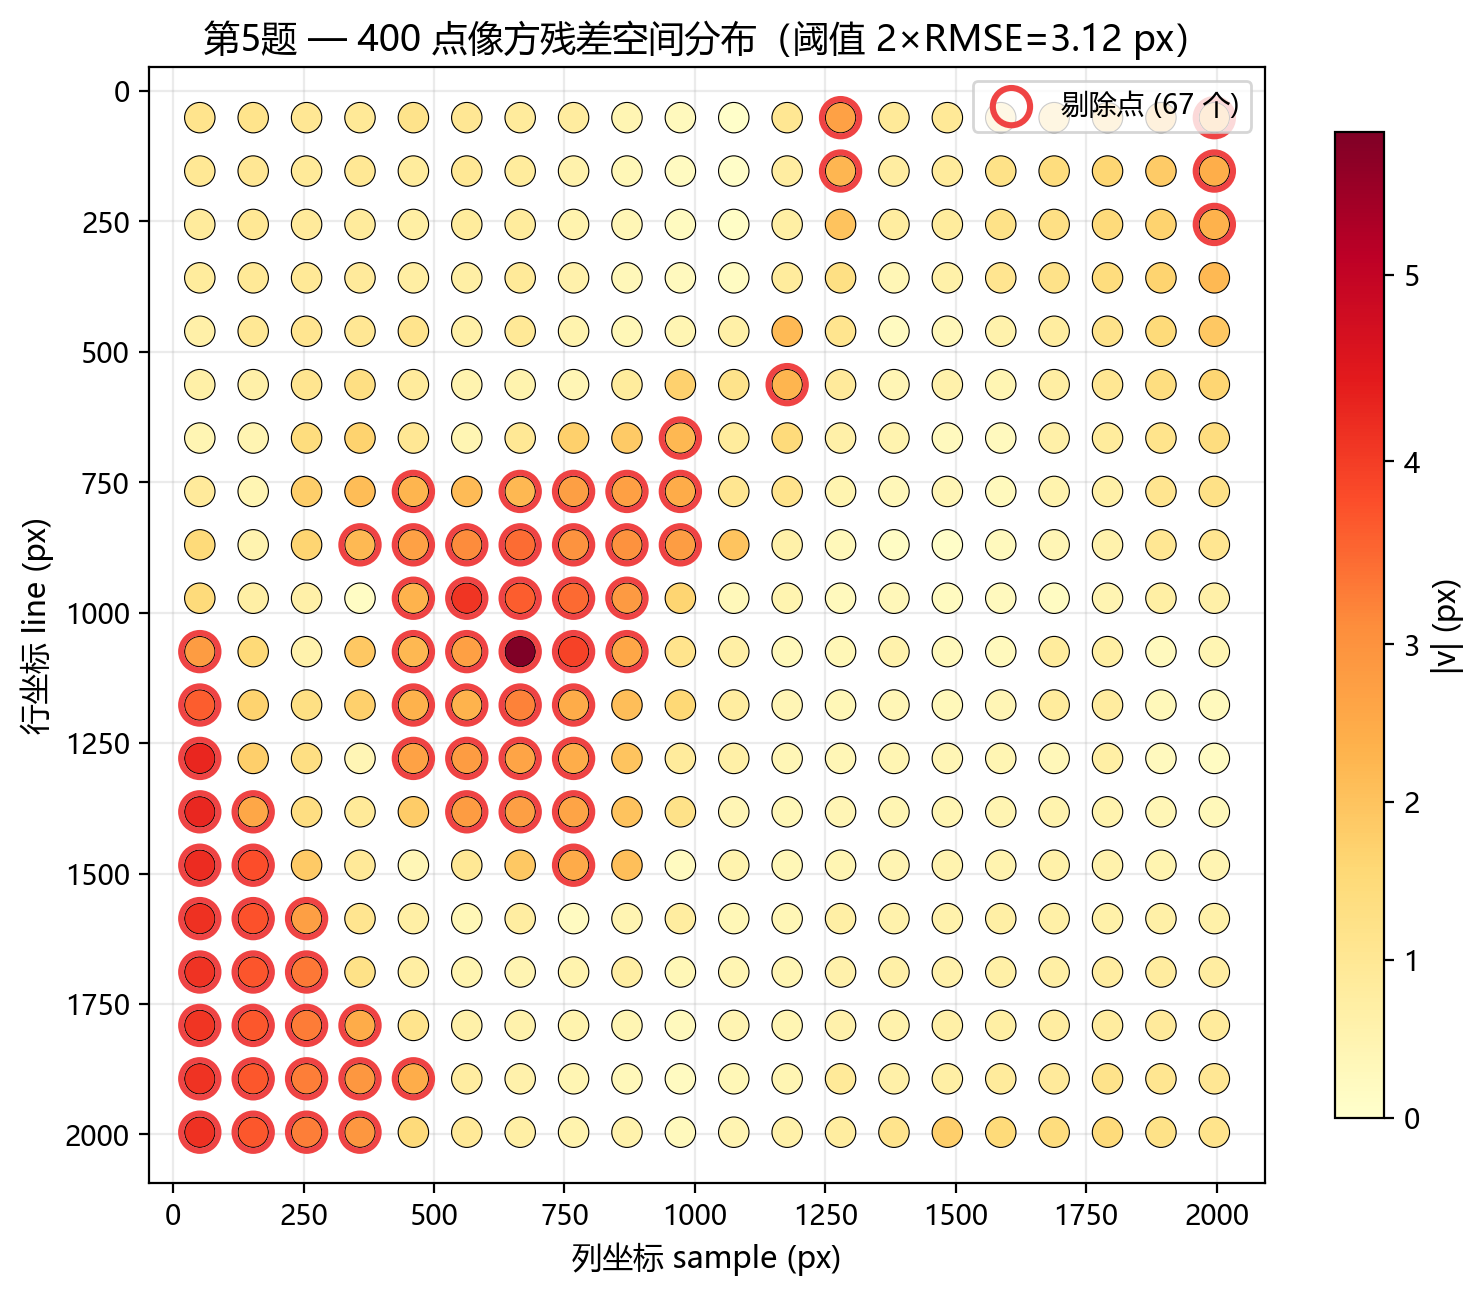
\includegraphics[width=0.88\textwidth]{figures/q5_residual_spatial_map.png}
  \caption{第 5 题 400 点像方残差空间分布（红圈为剔除点）}
  \label{fig:q5-spatial}
\end{figure}

\begin{figure}[H]
  \centering
  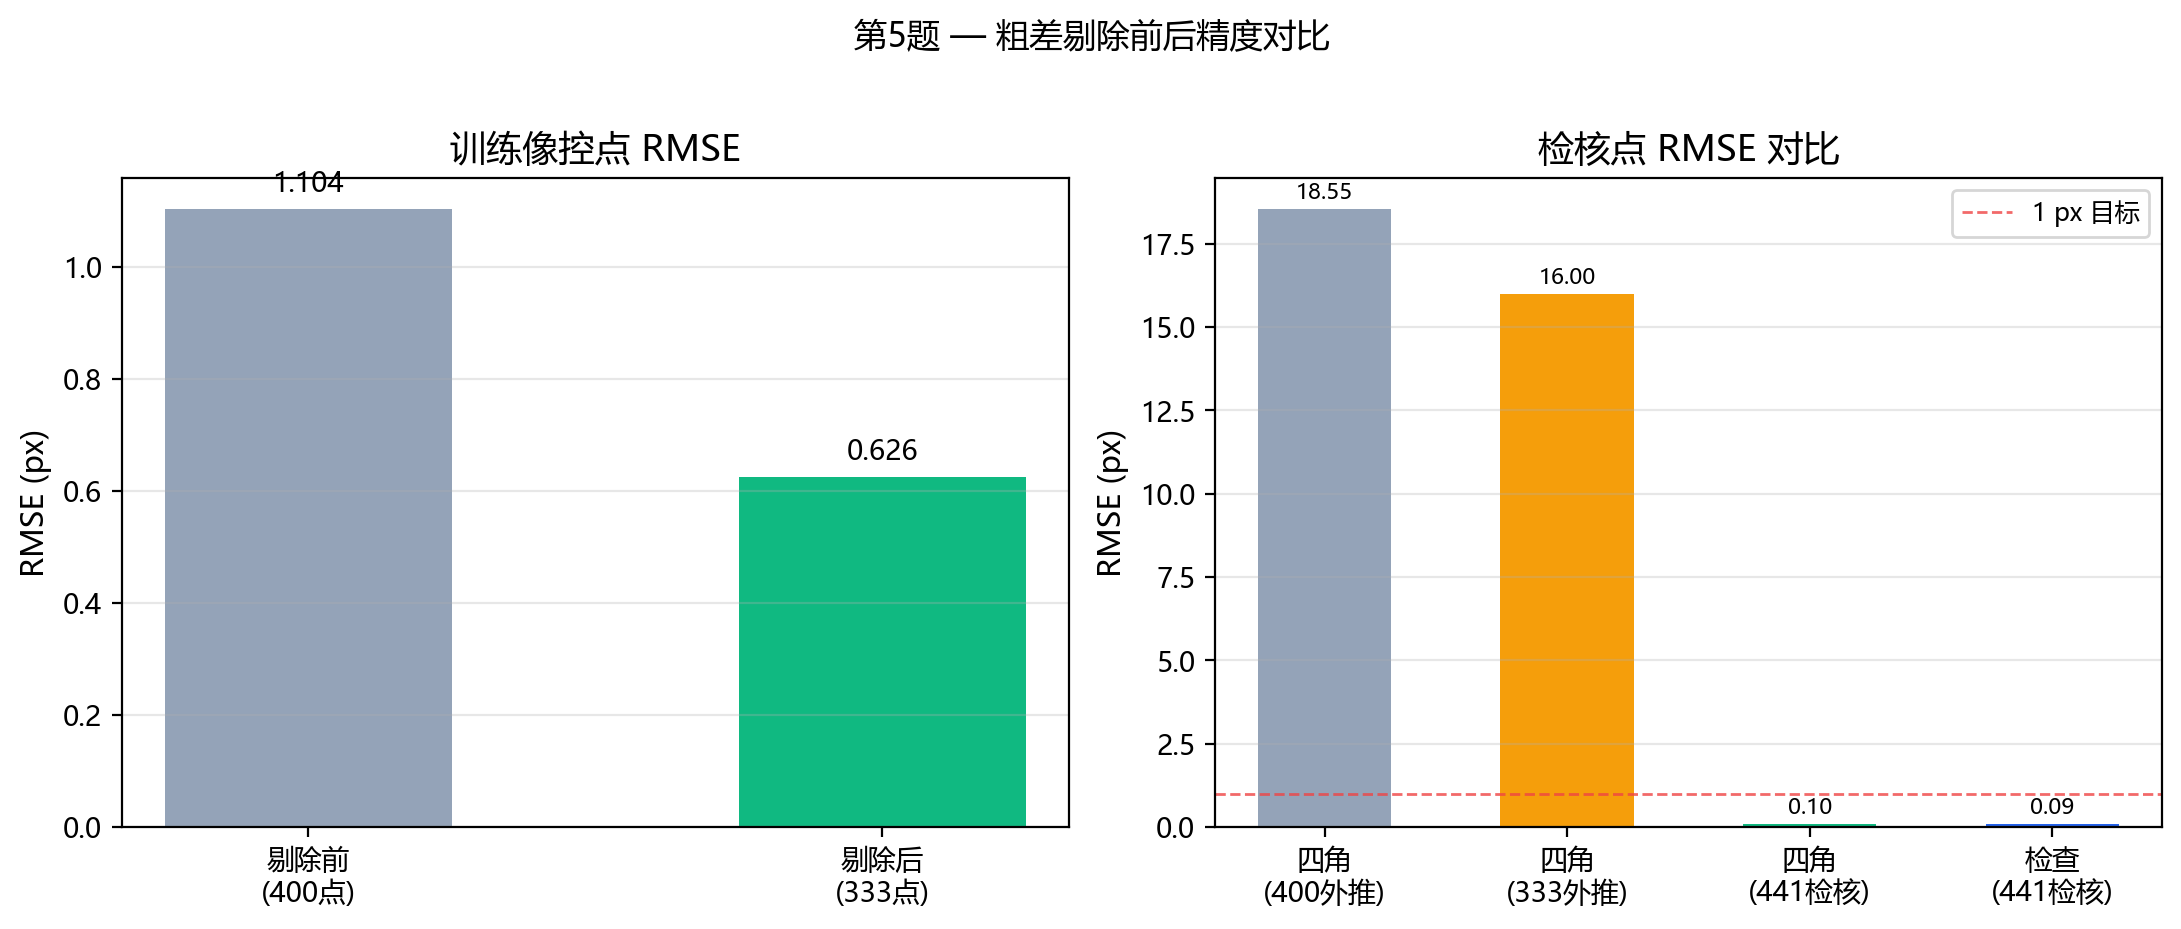
\includegraphics[width=0.88\textwidth]{figures/q5_before_after_rmse.png}
  \caption{第 5 题粗差剔除前后精度对比}
  \label{fig:q5-rmse}
\end{figure}

\subsection{实验结果分析（可选）}

441 点仿射检核达成 $<1$ px；训练 RMSE 从 1.10 px 降至 0.63 px。外推四角 RMSE 仍约 16 px，333 点仿射在影像边缘泛化不足，指导书允许此情况。67 个剔除点集中于城市建成区，残差方向以列方向为主，符合建筑物投影差特征。

% =============================================================================
\section{实习总结和感想}

通过 Task2 的五道题，完成了从官方像控点 RPC 精化、影像匹配加密、DEM/椭球高补全高程、到建筑物粗差剔除的完整工程链路。主要收获如下：

\begin{enumerate}
  \item \textbf{高程基准至关重要：}Q3 与 Q4 的对比说明，正高与椭球高混用会导致四角 RMSE 从 0.1 px 恶化到 7.7 px；EGM2008 高程异常修正是高精度 RPC 精化的必要步骤。
  \item \textbf{检核方法须正确：}400 点训练的仿射参数不能用于检核 441 官方点；应独立用 441 点估计仿射、检核高程用参考椭球高。
  \item \textbf{粗差识别与投影差：}建筑物匹配点因 DEM 不含地物高度而产生投影差，后验 $2\times\mathrm{RMSE}$ 残差检验是有效的粗差剔除手段。
\end{enumerate}

\begin{table}[H]
  \centering
  \caption{Task2 各题精度达成情况汇总}
  \label{tab:summary}
  \begin{tabular}{>{\centering\arraybackslash}p{1.2cm}
                  >{\centering\arraybackslash}p{4.5cm}
                  >{\centering\arraybackslash}p{3cm}
                  >{\centering\arraybackslash}p{2.5cm}
                  >{\centering\arraybackslash}p{1.5cm}}
    \toprule
    题号 & 主要指标 & 结果 & 要求 & 达成 \\
    \midrule
    Q1 & 441 点 RMSE & 0.097 px & $<0.1$ px & $\checkmark$ \\
    Q2 & 加密点 / 内点 & 400 / 370 & 匹配图平行 & $\checkmark$ \\
    Q3 & 四角 RMSE（正高 DEM） & 7.70 px & $\sim$20 px & $\checkmark$ \\
    Q4 & 检查/四角 RMSE & 0.093 / 0.101 px & $<2$ px & $\checkmark$ \\
    Q5 & 检查/四角 RMSE & 0.093 / 0.101 px & $<1$ px & $\checkmark$ \\
    \bottomrule
  \end{tabular}
\end{table}

代码采用模块化设计（\texttt{rpc\_utils.py} 复用 Q1 核心函数），便于 Q3--Q5 串联执行，也为后续 Task3 及正射纠正奠定了基础。

\end{document}
